%% notes-tex/019-simb-multimodal-expression/sections/3-baselines.tex
%% SOURCE: results/expression_baselines_split/seed<k>.json and seed0_fold90.json
%% (expression_baselines_split.py, GilaHyper CPU job 1806, 2026-09-13);
%% results/expression_baselines_split/summary.json and the two generated tables
%% (expression_baselines_split_table.py); results/knn_embedding_probe.json
%% (knn_embedding_probe.py); results/split_indices_manifest.json (make_split_indices.py);
%% the v12 numbers from results/head_round_readout.csv; the full embedding study from
%% results/baselines_split_fig3_proteome_full/ and results/expression_baselines_split_full/
%% (expression_baselines_split.py --embedding-set full, GilaHyper CPU jobs 2264 and 2268,
%% 2026-09-16), summarized by baselines_embedding_study.py into
%% results/baselines_embedding_study.json, the generated table and the figure.

\section{The linear and neighbor baselines, on the partitions the model trains on
\secstatus{todo}}
\label{sec:baselines}

The four baselines of \cref{tab:strand-baselines} were scored on a private permutation of
the raw Kemmeren panel, so baseline and trained arm shared a task but not a partition.
Everything in this section reads the partition file the training run reads: for split seed
$k$ the \file{CellDataModule} writes \file{index_details_seed_k.json}, the record indices
per split, and both the baseline script and the GPU launcher take that file as given. The
files are hashed in \file{split_indices_manifest.json}; seeds 0 to 2 carried the same hash
on both machines and seed 3 was built once and copied. The trained arms on the same four
partitions are the v13 round (\cref{sec:next}), running as this is written; nothing about
them is reported here.

\pfstep{Setup} Strain $b$ carries deletion set $S_b$ and a profile $y_b \in \mathbb{R}^F$
over $F = 6{,}169$ reporters, each entry the $\log_2$ ratio to the wild-type reference. The
partition $(\mathcal{T}, \mathcal{V}, \mathcal{E})$, train, validation, test, is the
datamodule's record-level 80/10/10 draw for split seed $k$: a seeded shuffle within each
index key (phenotype label, perturbation count), the per-key splits intersected. Every
deleted gene appears once in the panel, so every strain in $\mathcal{V}$ and $\mathcal{E}$
is an unseen perturbation. Per-gene training mean $\mu_f = |\mathcal{T}|^{-1}
\sum_{b \in \mathcal{T}} y_{bf}$ and residual $r_{bf} = y_{bf} - \mu_f$. The metric is the
training metric,
%
\begin{equation}
  \mathrm{pf}(\hat{Y}, Y)
  = \frac{1}{|\mathcal{F}_{\mathrm{ok}}|} \sum_{f \in \mathcal{F}_{\mathrm{ok}}}
    \frac{\langle \hat{y}_{\cdot f} - \bar{\hat{y}}_f,\; y_{\cdot f} - \bar{y}_f \rangle}
         {\|\hat{y}_{\cdot f} - \bar{\hat{y}}_f\|\,\|y_{\cdot f} - \bar{y}_f\|},
  \qquad
  \mathrm{nmse}(\hat{Y}, Y) = \frac{\sum_{b,f} (\hat{y}_{bf} - y_{bf})^2}
                                   {\sum_{b,f} (y_{bf} - \mu_f)^2},
  \label{eq:pf}
\end{equation}
%
with the columns and the means taken over the strains of the scored split and
$\mathcal{F}_{\mathrm{ok}}$ the reporters whose prediction and target both have a norm
above $10^{-8}$. A prediction constant across strains has no surviving column and scores
exactly $0$, which is what makes the first two baselines a self-check rather than a
competitor.

\pfstep{B0 and B1} $\hat{y}_{bf} = \mu_f$ and $\hat{y}_{bf} = 0$. Both are $0$ on
\cref{eq:pf} on every partition; B0's \file{nmse} is $1$ by construction, and the script
raises if either lands elsewhere. B1's \file{nmse} is how far the panel sits from the
reference: $1.33$, $1.33$, $1.37$ and $1.39$ on the validation strains of splits 0 to 3.

\pfstep{B2, the bilinear ridge} The perturbation is represented by an external gene
embedding, $p_b = |S_b|^{-1} \sum_{g \in S_b} e_g \in \mathbb{R}^D$, standardized column by
column on the training strains; a strain with no embedded gene is excluded from the score
and counted. The gene basis $G \in \mathbb{R}^{F \times K}$ holds the top-$K$ right singular
vectors of the training residual matrix $R_{\mathcal{T}}$, and
%
\begin{equation}
  W^{\star} = \operatorname*{argmin}_{W}
    \big\| R_{\mathcal{T}} G - P_{\mathcal{T}} W \big\|_F^2 + \lambda \|W\|_F^2
  = \big( P_{\mathcal{T}}^{\top} P_{\mathcal{T}} + \lambda I \big)^{-1}
    P_{\mathcal{T}}^{\top} R_{\mathcal{T}} G,
  \qquad
  \hat{Y} = P\, W^{\star} G^{\top} + \mathbf{1} \mu^{\top}.
  \label{eq:b2}
\end{equation}
%
This is the benchmark's $Y \approx G W P^{\top} + b$ with the intercept removed by
centering. $K \in \{1, 2, 4, 8, 16, 32, 33, 64, 128, 256\}$ and
$\lambda \in \{10^{-3}, \ldots, 10^{2}\}$, sixty cells, chosen on validation.

\pfstep{B3, the neighbor mean} With $s_{bj} = \cos(p_b, p_j)$ over training strains $j$ and
$N_k(b)$ the $k$ largest, $\hat{r}_b = k^{-1} \sum_{j \in N_k(b)} r_j$ and
$\hat{y}_b = \hat{r}_b + \mu$, $k \in \{1, 3, 5, 10, 25\}$ chosen on validation. No fitted
parameter.

\pfstep{The kNN probe, the same idea on raw profiles} The earlier probe
(\file{knn_embedding_probe.py}) predicts the whole profile rather than the residual,
weights the neighbors by their clipped similarity, and ran on the split-0 partition file
before any of this existed, so it is already on the model's partition:
%
\begin{equation}
  \hat{y}_b = \sum_{j \in N_k(b)} w_{bj}\, y_j,
  \qquad
  w_{bj} = \frac{[s_{bj}]_+}{\sum_{j' \in N_k(b)} [s_{bj'}]_+},
  \qquad
  s_{bj} = \cos(e_b, e_j),
  \label{eq:knn}
\end{equation}
%
over fourteen embeddings and random embeddings of matched dimension as the floor. Its
validation set is the 140 single-deletion strains of split 0.

\pfstep{Selection mirrors the model's} A trained arm reports the epoch that maximizes
validation Pearson, an optimistic order statistic over epochs. B2's cell and B3's $k$ are
likewise the validation maximum, over sixty and five cells, so the validation columns below
carry the same kind of optimism as \file{roll_max}, and the test columns are the read that
does not. The 90/10 column folds the test records into train against the same validation
strains, the linear analog of the round's 90/10 arm, and has no test read.

%% GENERATED by experiments/019-simb-multimodal/scripts/expression_baselines_split_table.py
%% from results/expression_baselines_split/seed<k>.json and seed0_fold90.json
%% (expression_baselines_split.py). Do not edit by hand.
%% SOURCE: results/expression_baselines_split/*.json via expression_baselines_split_table.py
\begin{table}[htbp]
  \centering
  \footnotesize
  \caption[Linear and neighbor baselines on the model's partitions]{\texttt{B2} and \texttt{B3} on the four \file{CellDataModule} partitions the v13 round trains on, \file{pearson_per_feature} on val and on test, where rank, ridge and $k$ are chosen on val and test is read at the chosen cell. Each partition has 1244 training strains and 155, 151, 155, 155 val (155, 150, 155, 155 test) labeled expression strains. The last column is split 0 with the test records folded into train (1399 training strains, the same val set), the linear analog of the round's 90/10 arm. \texttt{B0} is $0$ and \texttt{B1} is $0$ on every partition by construction; \texttt{B1}'s val \file{nmse} is 1.330, 1.327, 1.372, 1.391 on splits 0 to 3. \src{experiments/019-simb-multimodal/scripts/expression_baselines_split.py}}
  \label{tab:baselines-split}
  \setlength{\tabcolsep}{3.5pt}
  \begin{tabular}{@{}lllrrrrrr@{}}
    \toprule
     &  &  & \multicolumn{4}{c}{split seed} & mean $\pm$ sd & 90/10 \\
    \cmidrule(lr){4-7}
    baseline & embedding & read & 0 & 1 & 2 & 3 &  & val \\
    \midrule
    B2 bilinear ridge & ProtT5 & val & $+0.135$ & $+0.076$ & $+0.117$ & $+0.094$ & $0.106 \pm 0.026$ & $+0.137$ \\
     &  & test & $+0.085$ & $+0.148$ & $+0.111$ & $+0.097$ & $0.110 \pm 0.027$ & -- \\
    B2 bilinear ridge & CaLM & val & $+0.098$ & $+0.081$ & $+0.080$ & $+0.099$ & $0.089 \pm 0.010$ & $+0.102$ \\
     &  & test & $+0.069$ & $+0.120$ & $+0.087$ & $+0.093$ & $0.092 \pm 0.021$ & -- \\
    B2 bilinear ridge & species LM & val & $+0.043$ & $+0.044$ & $+0.022$ & $+0.042$ & $0.038 \pm 0.010$ & $+0.044$ \\
     &  & test & $+0.061$ & $+0.019$ & $+0.017$ & $+0.060$ & $0.040 \pm 0.024$ & -- \\
    B2 bilinear ridge & chromatin pathways & val & $+0.107$ & $+0.032$ & $+0.036$ & $+0.036$ & $0.053 \pm 0.036$ & $+0.110$ \\
     &  & test & $+0.004$ & $+0.040$ & $+0.031$ & $+0.006$ & $0.020 \pm 0.018$ & -- \\
    \midrule
    B3 neighbor mean & ProtT5 & val & $+0.130$ & $+0.113$ & $+0.111$ & $+0.126$ & $0.120 \pm 0.009$ & $+0.141$ \\
     &  & test & $+0.046$ & $+0.162$ & $+0.124$ & $+0.142$ & $0.118 \pm 0.051$ & -- \\
    B3 neighbor mean & CaLM & val & $+0.122$ & $+0.092$ & $+0.072$ & $+0.117$ & $0.101 \pm 0.023$ & $+0.123$ \\
     &  & test & $+0.088$ & $+0.115$ & $+0.086$ & $+0.111$ & $0.100 \pm 0.015$ & -- \\
    B3 neighbor mean & species LM & val & $+0.061$ & $+0.101$ & $+0.029$ & $+0.056$ & $0.062 \pm 0.030$ & $+0.070$ \\
     &  & test & $+0.045$ & $+0.050$ & $+0.041$ & $+0.056$ & $0.048 \pm 0.006$ & -- \\
    B3 neighbor mean & chromatin pathways & val & $+0.063$ & $+0.020$ & $+0.016$ & $+0.032$ & $0.033 \pm 0.021$ & $+0.058$ \\
     &  & test & $-0.008$ & $+0.011$ & $+0.003$ & $+0.003$ & $0.002 \pm 0.008$ & -- \\
    \bottomrule
  \end{tabular}
\end{table}


%% GENERATED by experiments/019-simb-multimodal/scripts/expression_baselines_split_table.py
%% from results/knn_embedding_probe.json (knn_embedding_probe.py). Do not edit by hand.
%% SOURCE: results/knn_embedding_probe.json via expression_baselines_split_table.py
\begin{table}[htbp]
  \centering
  \footnotesize
  \caption[The kNN embedding probe on expression]{The parameter-free neighbor probe on expression: a held-out deletion's profile predicted as the similarity-weighted mean of the profiles of its $k$ nearest other deleted genes in the embedding space named, \file{pearson_per_feature} on the 140 single-deletion validation strains of split seed 0, best $k$ over $\{1, 3, 5, 10, 25, 50\}$ and three fixed $k$. Dimension in parentheses. The random rows are embeddings of matched dimension drawn once, and set the floor. One-hot is undefined (every cosine similarity is zero) and is omitted. \src{experiments/019-simb-multimodal/scripts/knn_embedding_probe.py}}
  \label{tab:knn-probe}
  \begin{tabular}{@{}lrrrrr@{}}
    \toprule
    embedding (dim) & best $k$ & at best $k$ & $k{=}1$ & $k{=}10$ & $k{=}25$ \\
    \midrule
    ProtT5 (1,024) & 25 & $+0.117$ & $+0.065$ & $+0.091$ & $+0.117$ \\
    ESM2 650M (1,280) & 50 & $+0.092$ & $+0.064$ & $+0.080$ & $+0.083$ \\
    CaLM (768) & 25 & $+0.069$ & $+0.056$ & $+0.069$ & $+0.069$ \\
    codon frequency (64) & 50 & $+0.064$ & $+0.023$ & $+0.058$ & $+0.046$ \\
    chromatin pathways (197) & 3 & $+0.051$ & $+0.015$ & $+0.021$ & $+0.024$ \\
    species LM, both flanks (1,536) & 25 & $+0.014$ & $+0.009$ & $+0.005$ & $+0.014$ \\
    nucleotide transformer, both flanks (5,120) & 50 & $+0.012$ & $-0.017$ & $+0.004$ & $+0.009$ \\
    random (10) & 3 & $+0.011$ & $-0.000$ & $+0.003$ & $-0.006$ \\
    random (100) & 5 & $+0.018$ & $+0.014$ & $+0.016$ & $-0.011$ \\
    random (1,000) & 5 & $+0.033$ & $+0.008$ & $+0.016$ & $-0.001$ \\
    \bottomrule
  \end{tabular}
\end{table}


\pfstep{The partition moves a linear model as much as it moves the network} B2 on ProtT5
reads $0.135$, $0.076$, $0.117$ and $0.094$ on the four validation draws, a spread of
$0.026$ from a sixty-cell ridge with no seed of its own, and B3 on ProtT5 spreads $0.051$ on
test. The four draws share the same training count and differ in which 155 strains are
held out (the 72 Sameith doubles land 15, 13, 7 and 10 in validation), so the spread is the
partition itself. Eight more partitions, split seeds 4 to 11, exist only for the linear
models, and over the twelve draws B2 on ProtT5 reads $0.104 \pm 0.018$ on validation
(range $0.076$ to $0.135$) and $0.108 \pm 0.017$ on test; B3 on ProtT5 $0.122 \pm 0.020$
and $0.118 \pm 0.034$. Split 0 is the highest of the twelve validation draws for B2 and the
third highest for B3. That is the axis the v13 round was built to measure for the trained
arms, and the linear numbers say it is large before any network is involved.
\src{experiments/019-simb-multimodal/results/expression_baselines_split/summary.json}

\pfstep{Split 0 is the easiest validation draw for the linear models too} On split 0 both
ProtT5 baselines post their highest validation score of the four draws and B2 its lowest
test score, $0.085$ against $0.148$, $0.111$ and $0.097$ on the others; B3 on ProtT5 drops
from $0.130$ on validation to $0.046$ on test there. Every score the campaign has quoted is
a split-0 validation number. The v12 reference stack on that draw reads $0.174 \pm 0.008$
and \file{H_concat} $0.188 \pm 0.005$ at 1{,}399 epochs (\cref{sec:readouts-head}), against
$0.135$ for the best linear cell and $0.130$ for the best neighbor rule on the same 155
strains, so the margin over the linear model on this partition is $0.04$ to $0.05$, not the
$0.09$ that \cref{tab:strand-baselines} gave on a different permutation. The earlier
$0.104$ was not wrong; it was another draw.

\pfstep{Ten percent more training data buys the linear models almost nothing} With the 155
test strains folded into train, B2 on ProtT5 moves from $0.135$ to $0.137$ and B3 from
$0.130$ to $0.141$ on the same validation set, and CaLM by $+0.004$ and $+0.001$. Whether
the trained arms move more is what task 2 of the round measures; the linear result is the
floor that comparison is read against.

\pfstep{Embeddings rank the same way under every rule} ProtT5 leads B2, B3 and the probe on
every partition; CaLM is second; the species language model over both flanks sits at
$0.04$ to $0.06$; the chromatin-pathway feature fits validation on split 0 and transfers to
test at $0.004$ and $0.02$, the one case where the sixty-cell selection is visibly
optimistic. In the probe, every nucleotide-transformer arm is at or below the random floor
of $0.033$, and ProtT5's $0.117$ at $k = 25$ is what \cref{sec:strand-oracle} quotes.

\subsection{Every gene representation, on the proteome and on expression\secstatus{todo}}
\label{sec:baselines-embedding-study}

The gate above reads four representations. The v14 proteome round raised the question of
which representation of the deleted gene carries its protein response, and whether a
protein language model other than ProtT5, a DNA model, or a composite would move the
linear floor. So every representation the embedding builder serves was run as the
perturbation input of B2 and B3 on the same four partitions, for the proteome build
(3{,}581 training strains, 1{,}536 proteins after the coverage filter) and for the
expression build: two protein language models (ProtT5 and ESM2 650M, each with and
without the dubious ORFs), two coding-sequence representations (CaLM, codon frequency),
the species-aware fungal transformer over the 5' and 3' flanks, the Nucleotide
Transformer over six windows, the chromatin-pathway graph vector, random controls at
three widths, and eight composites including the four-embedding stack the trained model
consumes. \Cref{tab:baselines-embedding-study} and \cref{fig:baselines-embedding-study}
carry every number; the seed sd is $0.005$ to $0.012$ on the proteome and $0.01$ to
$0.03$ on expression, so a difference under about $0.02$ between two rows is not
resolved by four partitions.
\src{experiments/019-simb-multimodal/results/baselines_embedding_study.json}

\begin{figure}[htbp]
\centering
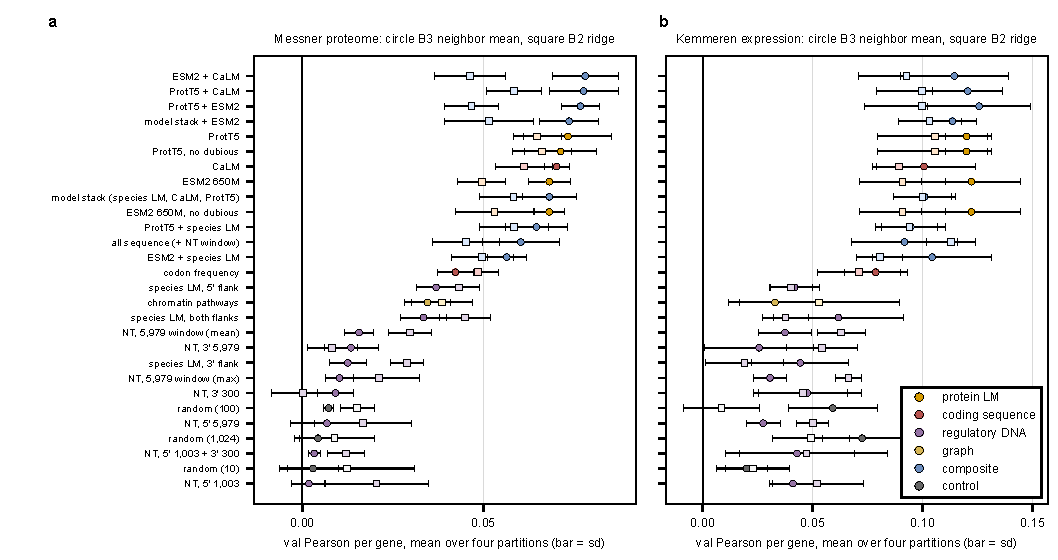
\includegraphics[width=\textwidth]{figures/baselines_embedding_study.pdf}
\caption[]{\textbf{Protein and coding-sequence representations carry the deleted gene's
response on both panels, no protein language model beats ProtT5, composites add nothing
the seed spread can resolve, and every regulatory-DNA representation sits at the random
floor.} \textbf{a}, the Messner proteome; \textbf{b}, Kemmeren expression. Each row is one
representation as the perturbation input of B3, the neighbor mean (circle), and B2, the
bilinear ridge (square); the point is the mean validation per-gene Pearson over the four
split partitions and the bar its sd. Rows ordered by the proteome's B3 mean; colors by
representation family. Generated by \file{baselines_embedding_study.py}.}
\label{fig:baselines-embedding-study}
\end{figure}

%% GENERATED by experiments/019-simb-multimodal/scripts/baselines_embedding_study.py
%% from results/baselines_split_fig3_proteome_full/ and results/expression_baselines_split_full/.
%% Do not edit by hand.
%% SOURCE: results/baselines_embedding_study.json via baselines_embedding_study.py
\begin{table}[htbp]
  \centering
  \footnotesize
  \caption[Every gene representation as the baseline's perturbation input]{Every gene representation the builder serves, as the perturbation input of the two embedding baselines on the four split partitions of the proteome and of the expression build. B2 is the bilinear ridge from the deleted gene's embedding (rank and ridge selected on val), B3 the mean profile of the $k$ nearest deleted genes in embedding space ($k$ selected on val). Val is the mean $\pm$ sd over the four seeds of the per-gene Pearson; test is the mean at the val-selected cell. Ordered by the proteome's B3 val mean. \src{experiments/019-simb-multimodal/scripts/baselines_embedding_study.py}}
  \label{tab:baselines-embedding-study}
  \setlength{\tabcolsep}{2.5pt}
  \begin{tabular}{@{}p{3.5cm}p{1.6cm}r rr rr rr rr@{}}
    \toprule
    & & & \multicolumn{4}{c}{proteome} & \multicolumn{4}{c}{expression} \\
    \cmidrule(lr){4-7} \cmidrule(lr){8-11}
    representation & family & dim & B2 val & test & B3 val & test & B2 val & test & B3 val & test \\
    \midrule
    ESM2 + CaLM & composite & 2,048 & $0.046 \pm 0.010$ & $0.053$ & $0.078 \pm 0.009$ & $0.075$ & $0.093 \pm 0.022$ & $0.099$ & $0.114 \pm 0.024$ & $0.104$ \\
    ProtT5 + CaLM & composite & 1,792 & $0.058 \pm 0.008$ & $0.061$ & $0.078 \pm 0.010$ & $0.081$ & $0.100 \pm 0.021$ & $0.106$ & $0.121 \pm 0.016$ & $0.108$ \\
    ProtT5 + ESM2 & composite & 2,304 & $0.047 \pm 0.008$ & $0.051$ & $0.077 \pm 0.005$ & $0.074$ & $0.100 \pm 0.026$ & $0.104$ & $0.126 \pm 0.023$ & $0.107$ \\
    model stack + ESM2 & composite & 4,608 & $0.052 \pm 0.012$ & $0.050$ & $0.074 \pm 0.008$ & $0.072$ & $0.103 \pm 0.014$ & $0.098$ & $0.114 \pm 0.011$ & $0.091$ \\
    ProtT5 & protein LM & 1,024 & $0.065 \pm 0.007$ & $0.062$ & $0.073 \pm 0.012$ & $0.078$ & $0.106 \pm 0.026$ & $0.110$ & $0.120 \pm 0.009$ & $0.118$ \\
    ProtT5, no dubious & protein LM & 1,024 & $0.066 \pm 0.008$ & $0.056$ & $0.071 \pm 0.010$ & $0.079$ & $0.106 \pm 0.026$ & $0.110$ & $0.120 \pm 0.009$ & $0.118$ \\
    CaLM & coding sequence & 768 & $0.061 \pm 0.008$ & $0.064$ & $0.070 \pm 0.003$ & $0.070$ & $0.089 \pm 0.010$ & $0.092$ & $0.101 \pm 0.023$ & $0.100$ \\
    ESM2 650M & protein LM & 1,280 & $0.050 \pm 0.007$ & $0.056$ & $0.068 \pm 0.006$ & $0.062$ & $0.091 \pm 0.020$ & $0.101$ & $0.122 \pm 0.022$ & $0.093$ \\
    model stack (species LM, CaLM, ProtT5) & composite & 3,328 & $0.058 \pm 0.009$ & $0.055$ & $0.068 \pm 0.008$ & $0.067$ & $0.100 \pm 0.013$ & $0.089$ & $0.101 \pm 0.014$ & $0.091$ \\
    ESM2 650M, no dubious & protein LM & 1,280 & $0.053 \pm 0.011$ & $0.057$ & $0.068 \pm 0.004$ & $0.061$ & $0.091 \pm 0.020$ & $0.101$ & $0.122 \pm 0.022$ & $0.093$ \\
    ProtT5 + species LM & composite & 2,560 & $0.059 \pm 0.009$ & $0.052$ & $0.065 \pm 0.009$ & $0.058$ & $0.094 \pm 0.013$ & $0.083$ & $0.095 \pm 0.016$ & $0.077$ \\
    all sequence (+ NT window) & composite & 7,168 & $0.045 \pm 0.009$ & $0.048$ & $0.060 \pm 0.011$ & $0.055$ & $0.113 \pm 0.011$ & $0.099$ & $0.092 \pm 0.024$ & $0.080$ \\
    ESM2 + species LM & composite & 2,816 & $0.050 \pm 0.008$ & $0.051$ & $0.056 \pm 0.005$ & $0.052$ & $0.081 \pm 0.010$ & $0.084$ & $0.104 \pm 0.027$ & $0.083$ \\
    codon frequency & coding sequence & 64 & $0.049 \pm 0.006$ & $0.042$ & $0.042 \pm 0.005$ & $0.043$ & $0.071 \pm 0.019$ & $0.052$ & $0.079 \pm 0.014$ & $0.062$ \\
    species LM, 5' flank & regulatory DNA & 768 & $0.043 \pm 0.006$ & $0.037$ & $0.037 \pm 0.005$ & $0.034$ & $0.040 \pm 0.010$ & $0.041$ & $0.042 \pm 0.011$ & $0.033$ \\
    chromatin pathways & graph & 197 & $0.039 \pm 0.008$ & $0.046$ & $0.035 \pm 0.006$ & $0.031$ & $0.053 \pm 0.036$ & $0.020$ & $0.033 \pm 0.021$ & $0.002$ \\
    species LM, both flanks & regulatory DNA & 1,536 & $0.045 \pm 0.007$ & $0.036$ & $0.033 \pm 0.006$ & $0.032$ & $0.038 \pm 0.010$ & $0.040$ & $0.062 \pm 0.030$ & $0.048$ \\
    NT, 5,979 window (mean) & regulatory DNA & 2,560 & $0.030 \pm 0.006$ & $0.021$ & $0.016 \pm 0.004$ & $0.008$ & $0.063 \pm 0.011$ & $0.049$ & $0.037 \pm 0.012$ & $0.017$ \\
    NT, 3' 5,979 & regulatory DNA & 2,560 & $0.008 \pm 0.007$ & $0.008$ & $0.013 \pm 0.007$ & $0.003$ & $0.054 \pm 0.016$ & $0.023$ & $0.026 \pm 0.025$ & $0.011$ \\
    species LM, 3' flank & regulatory DNA & 768 & $0.029 \pm 0.005$ & $0.017$ & $0.013 \pm 0.005$ & $0.002$ & $0.019 \pm 0.018$ & $0.021$ & $0.044 \pm 0.022$ & $0.021$ \\
    NT, 5,979 window (max) & regulatory DNA & 2,560 & $0.021 \pm 0.011$ & $0.020$ & $0.010 \pm 0.004$ & $0.008$ & $0.066 \pm 0.006$ & $0.060$ & $0.031 \pm 0.008$ & $0.024$ \\
    NT, 3' 300 & regulatory DNA & 2,560 & $0.000 \pm 0.009$ & $0.001$ & $0.009 \pm 0.005$ & $0.003$ & $0.046 \pm 0.020$ & $0.029$ & $0.048 \pm 0.025$ & $0.016$ \\
    random (100) & control & 100 & $0.015 \pm 0.005$ & $0.010$ & $0.007 \pm 0.001$ & $0.003$ & $0.009 \pm 0.017$ & $0.011$ & $0.059 \pm 0.020$ & $0.037$ \\
    NT, 5' 5,979 & regulatory DNA & 2,560 & $0.017 \pm 0.013$ & $-0.018$ & $0.007 \pm 0.010$ & $0.005$ & $0.050 \pm 0.007$ & $0.008$ & $0.028 \pm 0.008$ & $0.021$ \\
    random (1,024) & control & 1,024 & $0.009 \pm 0.011$ & $-0.004$ & $0.004 \pm 0.005$ & $0.001$ & $0.049 \pm 0.018$ & $0.013$ & $0.073 \pm 0.018$ & $0.018$ \\
    NT, 5' 1,003 + 3' 300 & regulatory DNA & 5,120 & $0.012 \pm 0.005$ & $0.009$ & $0.003 \pm 0.002$ & $0.005$ & $0.047 \pm 0.037$ & $0.041$ & $0.043 \pm 0.026$ & $0.045$ \\
    random (10) & control & 10 & $0.012 \pm 0.019$ & $0.006$ & $0.003 \pm 0.007$ & $0.001$ & $0.023 \pm 0.017$ & $0.003$ & $0.020 \pm 0.010$ & $0.002$ \\
    NT, 5' 1,003 & regulatory DNA & 2,560 & $0.021 \pm 0.014$ & $0.008$ & $0.002 \pm 0.005$ & $0.005$ & $0.052 \pm 0.021$ & $0.044$ & $0.041 \pm 0.009$ & $0.016$ \\
    \bottomrule
  \end{tabular}
\end{table}


\pfstep{The proteome floor is $0.07$ to $0.08$, and it is a protein-sequence floor} On the
proteome B3 reads $0.078$ for ESM2 with CaLM and for ProtT5 with CaLM, $0.077$ for ProtT5
with ESM2, $0.073$ for ProtT5 alone, $0.070$ for CaLM and $0.068$ for ESM2; B2 peaks at
$0.065$ on ProtT5. The two protein language models are level, and every composite lands
within $0.005$ of its best member. Below them codon frequency reads $0.042$, the species
language model over both flanks $0.033$, the chromatin-pathway vector $0.035$, and every
Nucleotide Transformer window $0.002$ to $0.016$ against random controls at $0.003$ to
$0.007$. The v14 arms at their matched epoch read $0.114$, $0.083$, $0.112$ and $0.085$
on the four partitions (\cref{sec:readouts-proteome}), so the trained model's margin over
the best linear floor is $0.00$ to $0.04$, and the floor was not raised by any
representation the gate had missed.

\pfstep{Expression reads the same order at twice the level} B3 on ProtT5 reads $0.120 \pm
0.009$ on validation and $0.118$ on test, ESM2 $0.122 \pm 0.022$ and $0.093$, ProtT5 with
ESM2 $0.126 \pm 0.023$ and $0.107$, CaLM $0.101$ and $0.100$; no composite beats ProtT5 on
test. The all-sequence composite (7{,}168 dimensions) reads the highest B2 validation of
the study, $0.113$, and $0.099$ on test, the width buying validation fit and not transfer.
The regulatory-DNA representations read $0.03$ to $0.06$ on validation and $0.01$ to
$0.05$ on test, where the 1{,}024-wide random control reads $0.073$ on validation and
$0.018$ on test; the neighbor rule in a random space fits the validation draw through its
choice of $k$ and transfers nothing, which is the size of the selection optimism on this
panel.

\pfstep{What this settles for the model} The input the trained model consumes, the
four-embedding stack, is not a better perturbation representation than ProtT5 alone under
either linear rule on either panel; the species-language-model flanks it carries are at
the random floor by themselves. ESM2 is a substitute for ProtT5, not an upgrade, and
adding it to the stack changes nothing a linear rule can see. The DNA models do not carry
the deletion response under these rules, on either panel, at any window. Whether the
network extracts something from the flanks that a bilinear map cannot is the embedding
factor's question (\cref{sec:readouts-factorial}); the linear answer is that there is nothing there to
extract at first order.
